%%%%%%%%%%%%%%%%%%%%%%%%%%%%%%%%%%%%%%%%%%%%%%%%%%%%%%%%%%%%%%%%%%%%%%%%%%%%%%%%%%%%%%%%%%%%%%%%%%%%%%
%
%   Filename    : chapter_4.tex 
%
%   Description : This file will contain your The Speech Feedback System.
%                 
%%%%%%%%%%%%%%%%%%%%%%%%%%%%%%%%%%%%%%%%%%%%%%%%%%%%%%%%%%%%%%%%%%%%%%%%%%%%%%%%%%%%%%%%%%%%%%%%%%%%%%

\chapter{The JLAD Feedback System}
This section gives the overall specifications and functional requirements of the software to be developed.

\section{System Overview}
JLAD aims to provide feedback for hearing-impaired students when pronouncing different combinations of consonants followed by diphthongs.

The teacher is provided with a range of training modules of a fixed set of consonant-diphthongs.  After the teacher selects a desired training module, the student can see himself through the webcam. Beside the webcam panel, the student is able to see a video of a teacher performing the correct mouth movements in which the student imitates. When the teacher fires the Record button, the student speaks through the microphone and JLAD will display the visual feedback of his pronunciation on how correct he is.

\begin{figure}[!htbp]
    \centering
    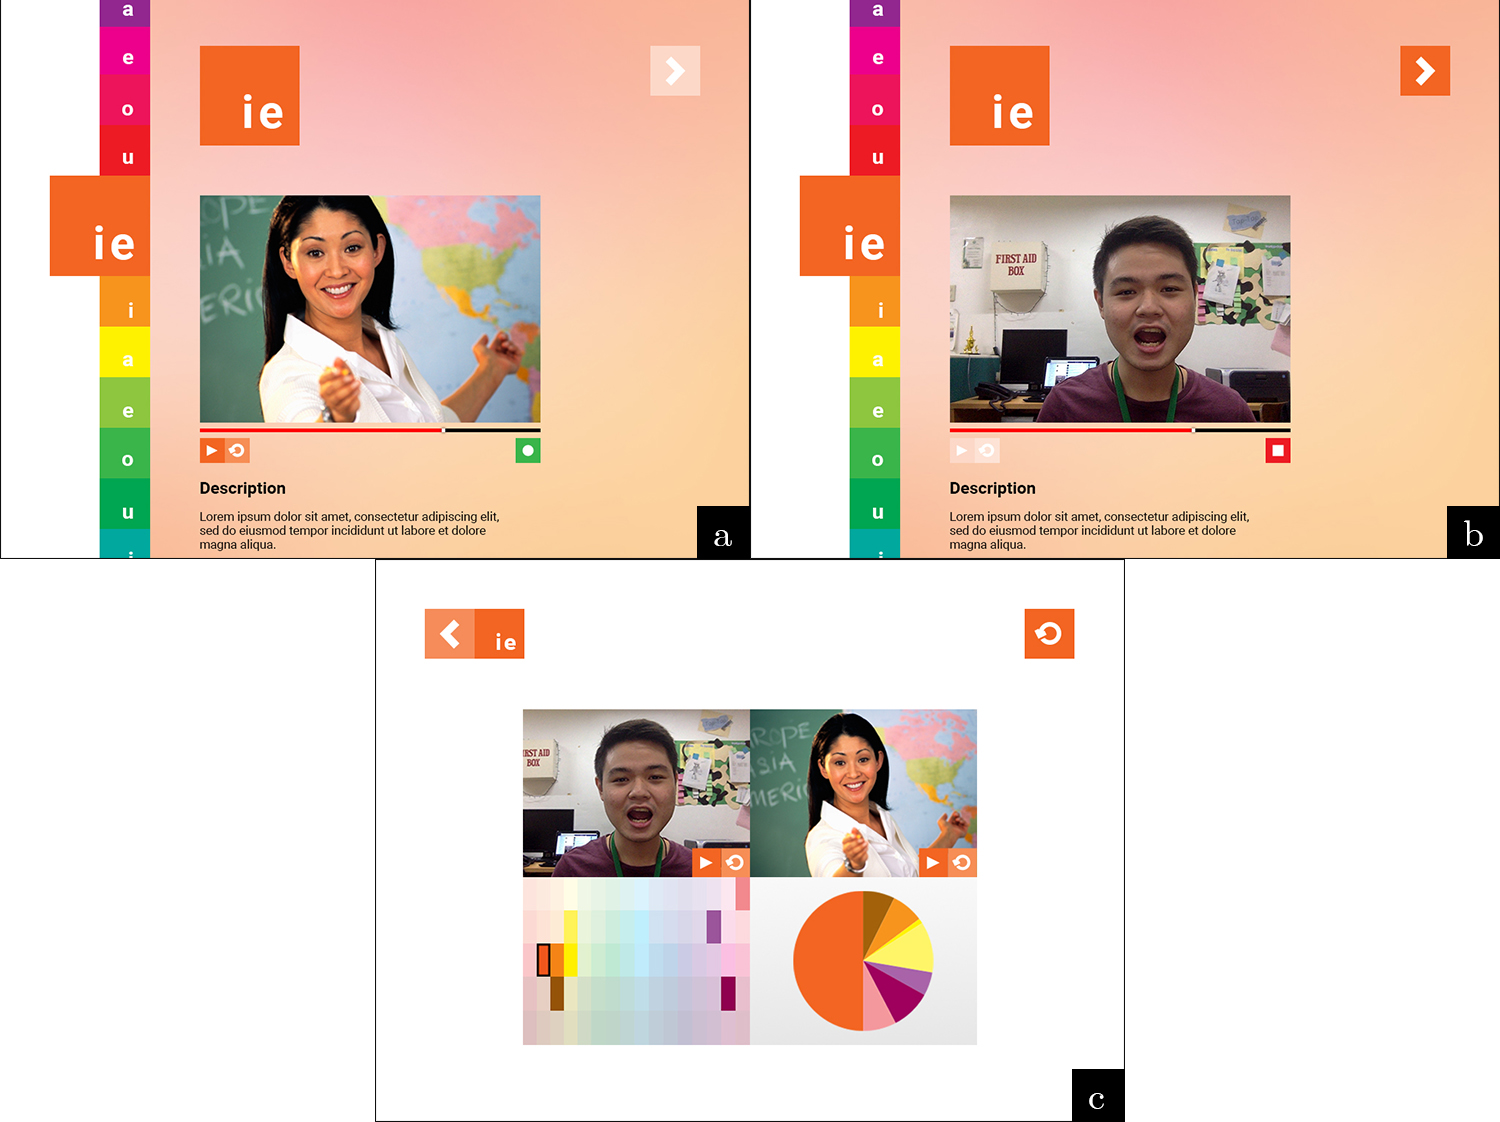
\includegraphics[totalheight=0.5\textheight]{UI}
    \caption{(A) The main menu allows the teacher to select a consonant-diphthong for the student to practice. (B) The teacher must record the student's pronunciation through the use of the record button. (C) After recording, the student is shown visual feedback displaying the sound he made in the spectrum along with his mouth movement}
    \label{fig:proto-mainmenu}
\end{figure}


\pagebreak

\section{System Objectives}

\subsection{General Objective}
To implement a feedback system for speech training that provides the user with correct mouth movement of a selected consonant-diphthong, to provide the user with a mean to see himself, and to provide measurable visual feedback.

\subsection{Specific Objectives}
\begin{enumerate}
\item To train the SOM into understanding consonant-diphthong pronunciations
\item To provide a visualization that shows feedback of the trainee's pronunciation of a consonant-diphthong combination
\item To deliver a video feedback for the speech trainee to see himself as reference as to how he performs different mouth movements
\item To display a video recording showing the speech trainee on how to perform the mouth movement of a selected consonant-diphthong combination
% \item To record the audio input of the trainee
\item To record a trainee's consonant-diphthong pronunciation
\item To have the system analyze the audio recording of the trainee and map it to the SOM
% REMOVE - Sir Sol \item To map the different diphthongs to their own corresponding color in the spectrum
\end{enumerate}

\section{System Scope and Limitations}
% How big is the dataset?
% What accents? Do accents matter?
% Are we going to use Desktop as our platform?
% What are we going to use it with?
% Is it stand-alone? With the assistance of a teacher?
The system will have a fixed set of consonant-diphthong combinations to be used for training which will be determined by the group. The diphthongs will be limited to what will be included in the SOM. The input will be compared only to the existing data, which means it will use the data to map the input as close as possible if it does not have a corresponding consonant-diphthong combination value. The system should be used by a trainee alongside a teacher or a speech therapist as the system may not be comprehensible enough to be used by a child alone. Also, the teacher may have to track the progress of their students.

Videos to be played in the system will be recorded videos of real teachers who will demonstrate correct mouth movement to their students. The webcam, designed to act as a student's reflection, should be running above 20 frames per second in order for the student to clearly observe their mouth movement. The webcam's resolution is set to a minimum of 320 by 240 pixels. The microphone requires to have at least 22050 Hz as its sampling rate. The audio is recorded in one channel only---mono. Only visual feedback will be considered in the system however the teacher may or should also provide feedback to their students by giving appraisal.

The system will only run on desktop and laptop machines with Java Runtime Environment (JRE) installed. The machine will need to have a microphone and a camera connected to it.

\pagebreak

\section{Architectural Design}

\subsection{Data Training}

\begin{figure}[h]
    \centering
    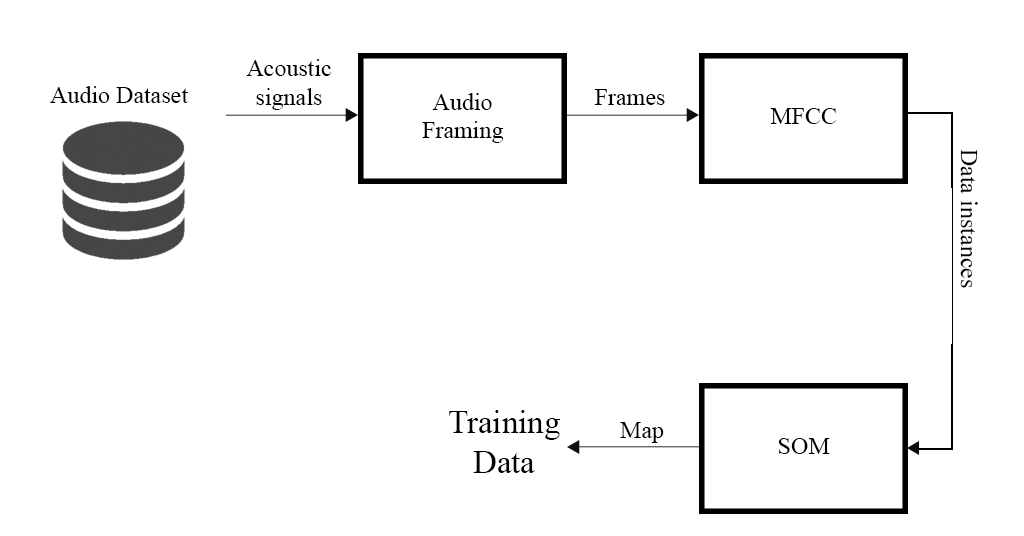
\includegraphics[totalheight=0.3\textheight]{diagram_training.png}
    \caption{System Architecture of the Data Training}
    \label{fig:architecture-training}
\end{figure}

To create a training model containing consonant-diphthong combinations for the feedback system, the researchers will adapt how Agustin's \citeyear{agustin:2014:SOM} created her training model. Recordings of consonant-diphthongs specified in the scope (see Chapter 1.3) will be collected as training data. Each acoustic signal are then split into frames of 16ms long with 5ms frame shift (defined in 3.2), similar to Agustin's configurations. The first 15 MFC coefficients are computed in each frame. The aforementioned data acquired is then fed into Agustin's SOM which produces a map. Each node of the SOM contains a subset of the whole training data \cite{agustin:2014:SOM}.

\subsection{Feedback System}

\begin{figure}[h]
    \centering
    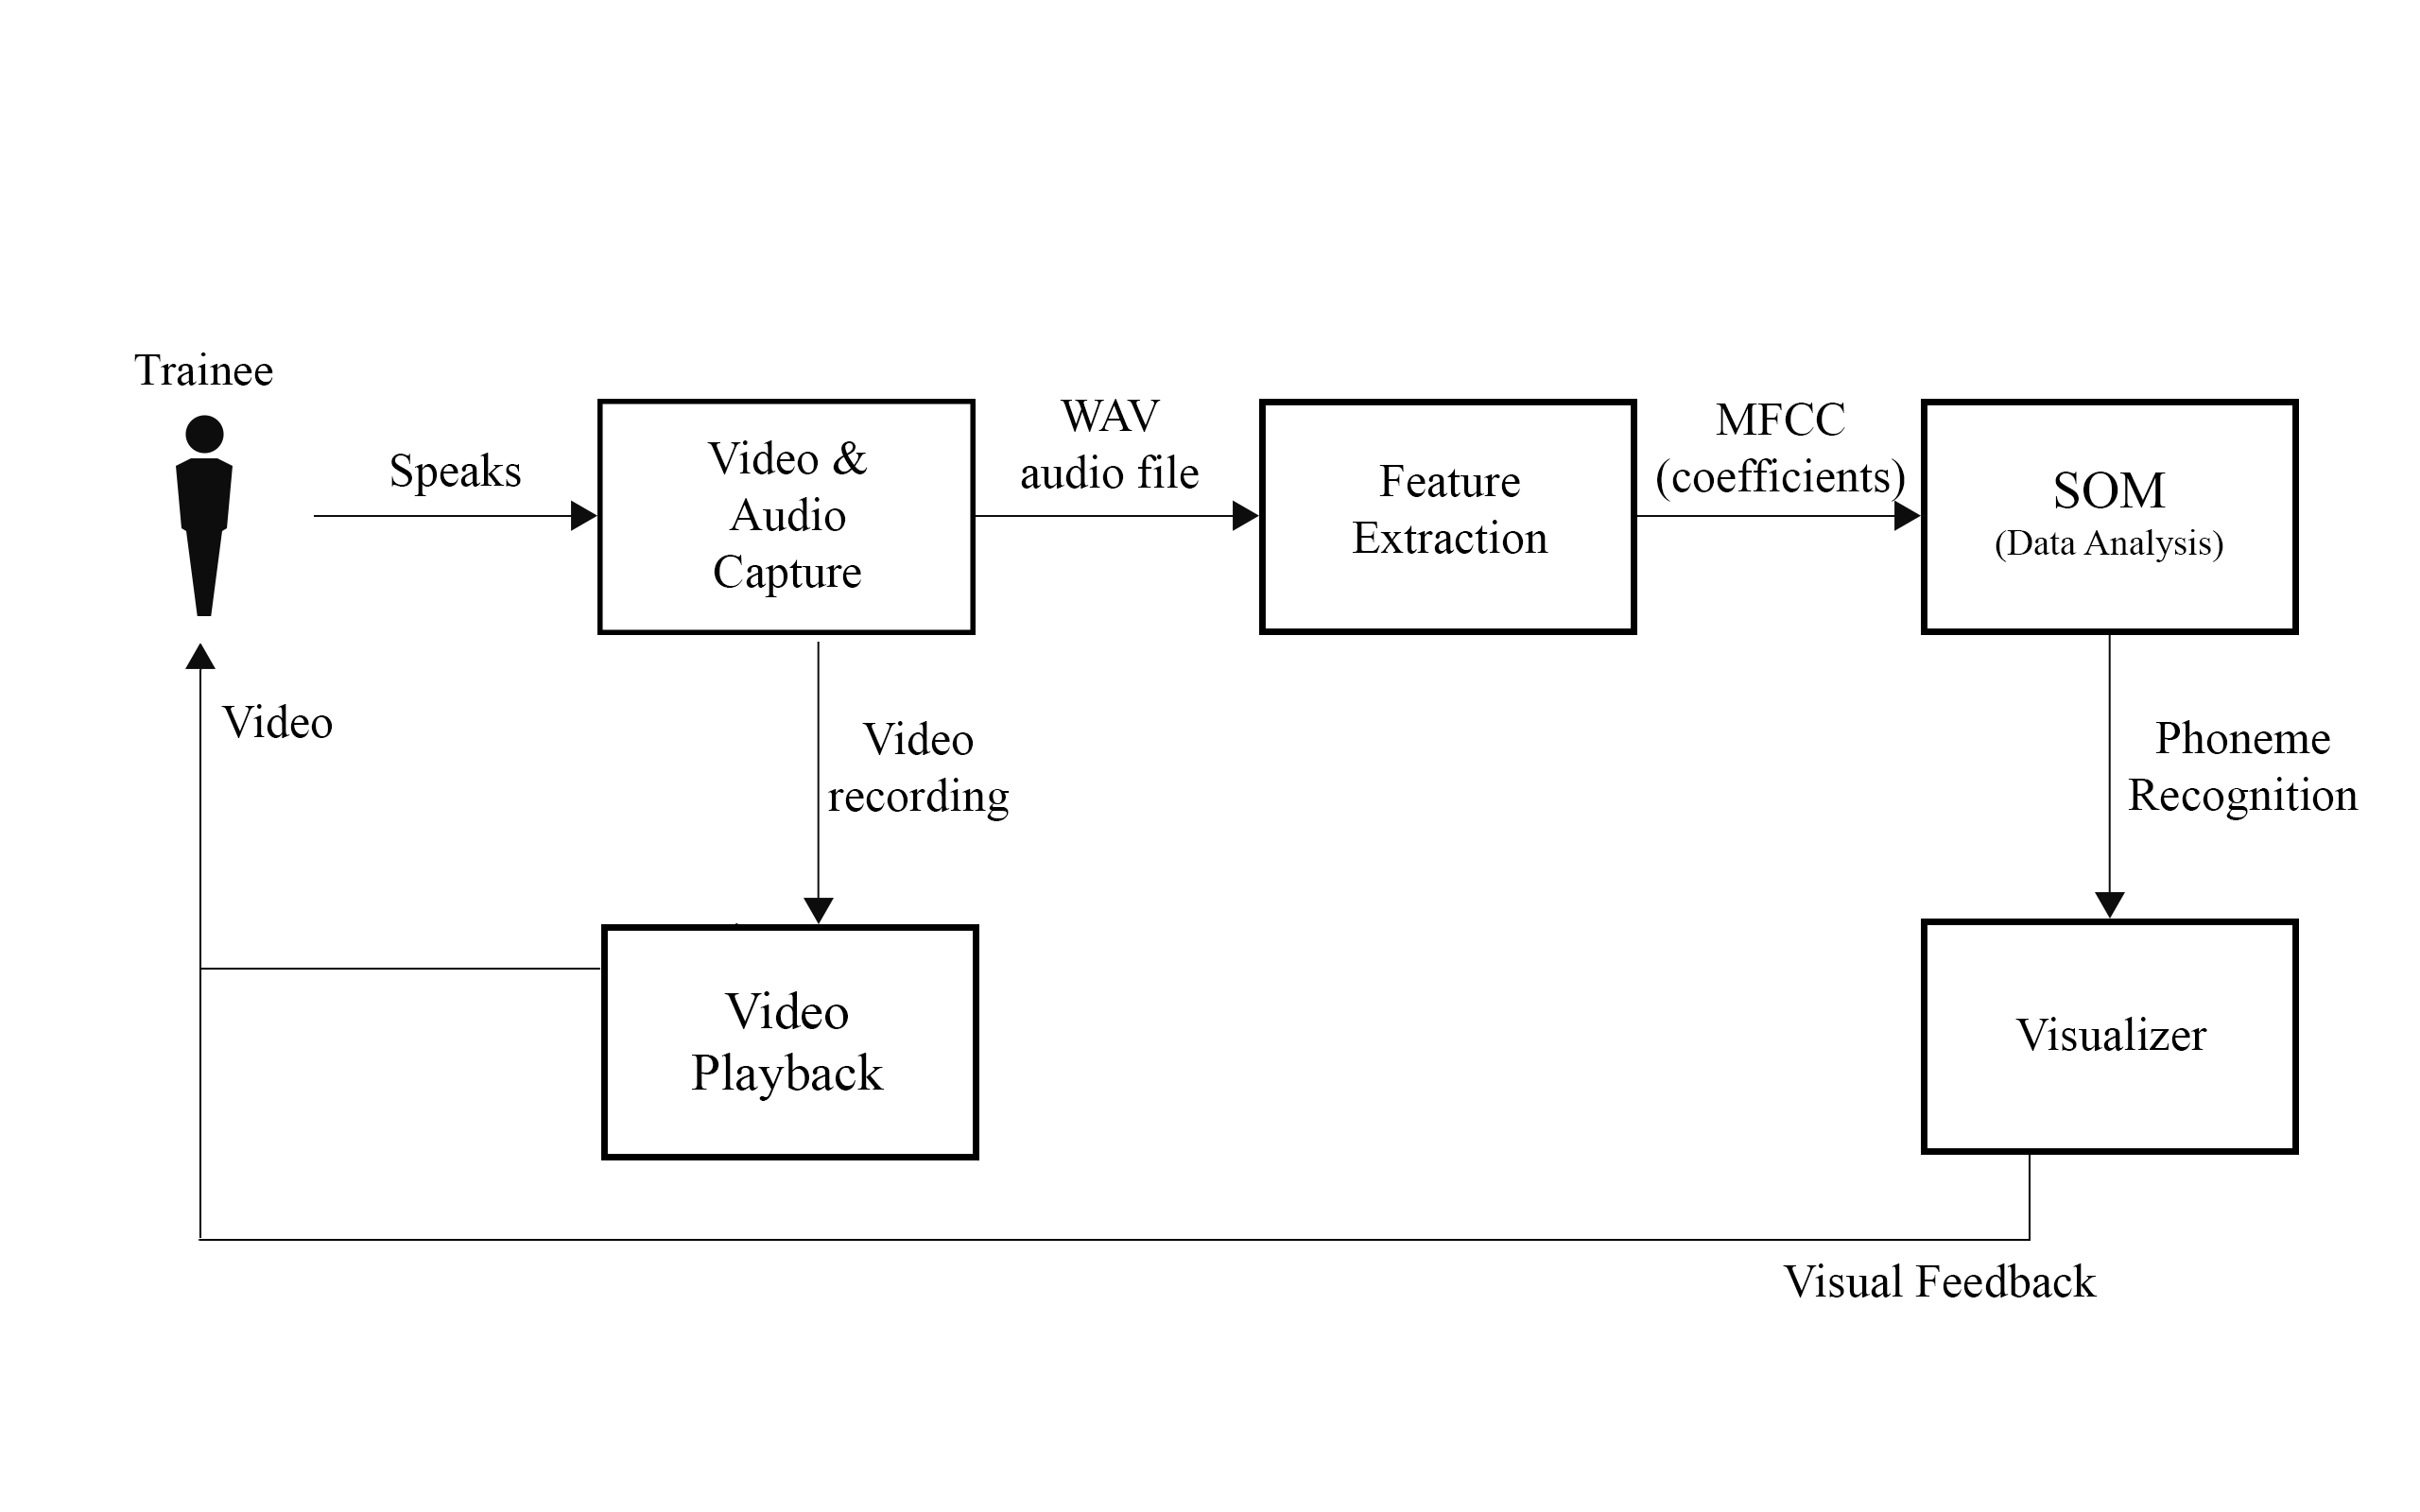
\includegraphics[totalheight=0.3\textheight]{diagram_v3.png}
    \caption{System Architecture of the Feedback System}
    \label{fig:architecture}
\end{figure}

The feedback system is composed of several modules. Each module has a significant responsibility in the feedback system, which greatly helps its users in producing correct speech. A live video camera showcasing the trainee's face will be displayed as well as a video playback of a teacher showing the proper mouth movement when pronouncing the target sound. The trainee interacts with the system in the Audio Capture module. After recording, the audio will go through Feature Extraction using MFCC, which translates important information from the audio into several coefficients. After Feature Extraction, the coefficients will then be laid out on the Self-Organizing Map, which determines how far or how near a trainee is from producing the target sound. The feedback will then be displayed to the trainee.
% Audio Recording -> Feature Extraction (MFCC) -> Mapping (SOM) -> Feedback Display

\section{System Functions}
This section discusses the functions or features available in the speech feedback system.

\subsection{Live Video Display}
For the trainee to see how well he is performing the correct mouth movement when speaking a certain consonant-diphthong combination, the proponents will display a live video display of the trainee which he or she will use for comparison with the recorded video (the correct mouth movement) beside it. This provides Interactive and Mode types of feedback as it visually shows what the student is currently doing.

\subsection{Video Player}
The purpose of the video player is to play a video recording that shows the user on how to correctly pronounce a certain consonant-diphthong combination in which the trainee must imitate. It will be placed beside the webcam display so that the trainee can compare and see if his mouth movement is similar to the video being played. This provides a Mode type of feedback as it shows a visual demonstration of what to do.

%audio record
\subsection{Record Audio}
For the software to process if the trainee's pronunciation is correct, it will need to record the pronunciation of the trainee. After recording, the software will process the voice input in order to display if the pronunciation is correct or not.

\subsection{Feedback Processing}
The software, having performed audio recording, will then process the audio into coefficients following the Mel-frequency cepstral coefficients (MFCC) model, which converts the audio recording into a readable format that will be accepted by the SOM.

After processing the audio and translating it into an array of coefficients, it will then be sent to the self-organizing map (SOM) which will classify the recording and then determine how far or how near the trainee's input is from the target pronunciation.

The software will determine and display how far or how near the trainee's pronunciation is from the target pronunciation through means of color representation. The representation is shown as a color spectrum or a color map. The feedback highlights a targeted color in the spectrum and where the student's pronunciation landed in the spectrum. The student may then keep trying until he gets the correct pronunciation by having the teacher record him again. This presents both the teacher and the student with Amount and Visual feedback (see \figref{fig:feedback-strategy-table} as it shows where and how near or how far the student is from the target pronunciation.

\section{Physical Environment and Resources}

\subsection{Hardware Resources}
The system runs on a desktop or a laptop machine. The system requires a microphone and a web camera connected to it. The minimum supported resolution of the system is 1024x768 pixels.

\subsection{Software}
%%java runtime environment
The machine needs to have the Java Runtime Environment version 1.8 installed for the feedback system to run.
%%vlc
The video player becomes functional when VLC media player is installed in the machine as the feedback system relies on VLC media player's libraries. It has to be noted that if the operating system is 32-bit, then a 32-bit version of VLC media player must be installed. A 64-bit OS will require a 64-bit version of VLC media player.
%%MATLAB
MATLAB is used to process the audio file (.wav) by using the Mel-frequency cepstral coefficients (MFCC) model which converts audio into coefficients. These coefficients are then saved to a comma separated value (CSV) file.
%%Java
Java will be the main programming language to develop the Speech Feedback system since Java is very flexible in terms of cross-platform, it can run on most operating systems.
%%list of libraries

%target users
%%